\subsection{研究方案和技术路线}

\begin{figure}[h]
    \begin{small}
        \begin{center}
            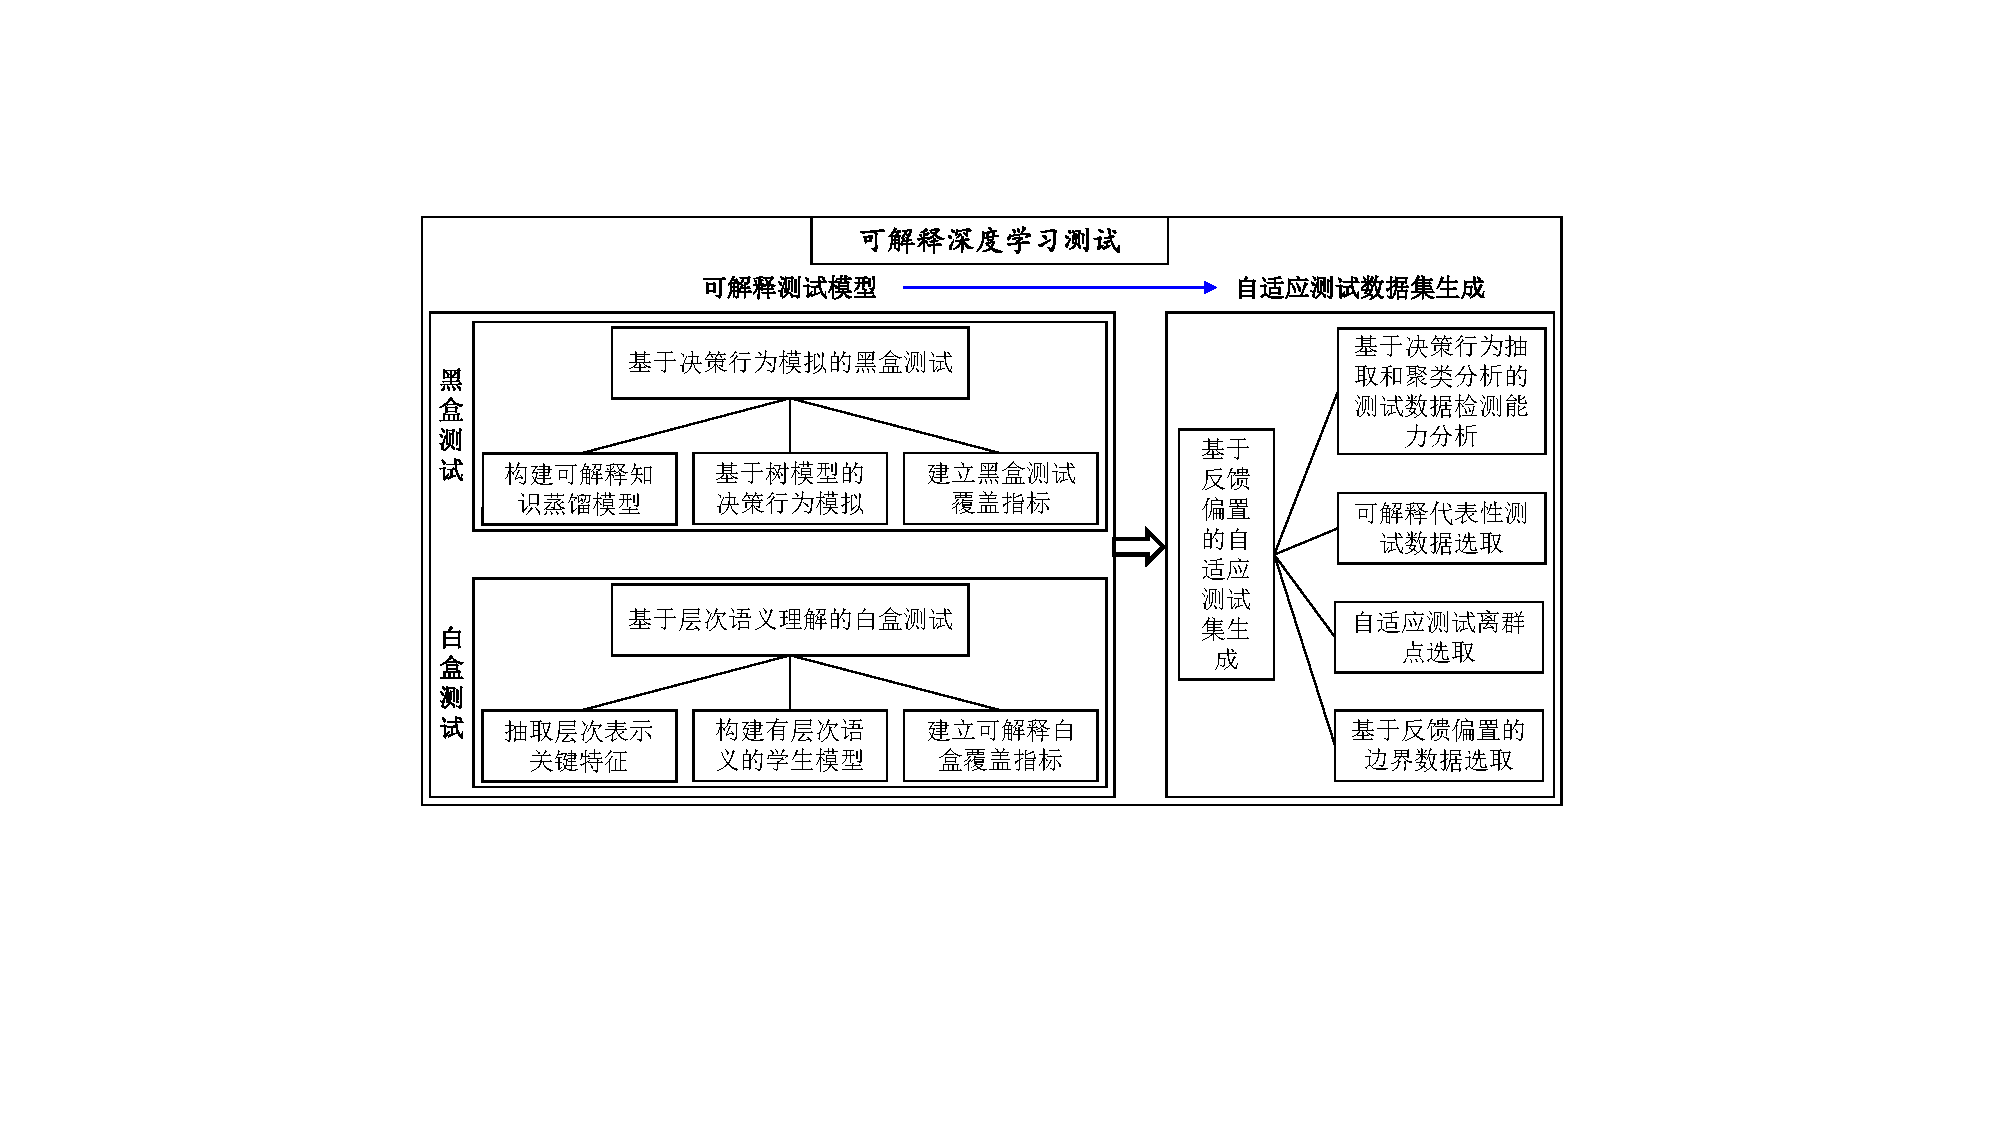
\includegraphics[width=0.95\textwidth]{ch3solution.pdf}
        \end{center}
        \caption{总体技术路线}
        \label{fig:ch3:solution}
    \end{small}
\end{figure}

围绕\ref{ch2content}规划的研究内容和\ref{ch2target}制定的研究目标,本项目拟定的
总体技术路线如\cref{fig:ch3:solution}所示。本项目针对电子医疗记录分析构建基于深
度学习的端到端的解决方案,通过对电子医疗记录数据集依次进行队列识别、EMR插补和可
解释预测,实现对特定患者队列的分析挖掘。本项目的主要研究内容分别对应大数据分析通
用流程中的数据获取、数据预处理和数据分析。此外,鉴于医疗领域的特殊性,本项目的研
究工作需要与医生进行充分的沟通,在模型设计和结果解释等方面融入医生的反馈。下面针
对各部分研究内容,详细介绍其具体研究方案和技术路线。



\subsubsection{基于表现型的自动队列识别}\label{ch3_1}

%要实现针对电子医疗记录的队列识别,首先需要构建患者的电子医疗记录表示学习模型,由
%于电子医疗记录特征维度高,本项目拟采用层次表示学习模型进行建模,同时,在模型中充
%分利用未标注数据,提高模型的学习效果。

\cref{fig:ch3:ci}展示了基于表现型的自动队列识别研究方案,如图所示,方案首先利用
RNN对电子医疗记录建模,得到患者不同时间点就医记录的向量表示。这一步有多种模型设
计选择,如采用双向RNN模型、加入注意力机制通常能得到更好表示学习结果,这对于本文
电子医疗记录建模非常重要,但序列建模的研究比较成熟,此处不再赘述。在得到患者的基
本表示$(\bm h_1, \bm h_2, \dots, \bm h_t)$后,以其作为上下文,在表现型字典$\bm
D$中查找相关的表现型向量(如图所示,即$\{\bm D_i\}$),同时得到表现型字典向量重
要性$\bm w$,以$\bm p = f(\{\bm D_i\}, \bm w)$作为患者的表现型表示。至此,
\textbf{构建了``特征$\rightarrow$一次就医$\rightarrow$表现型$\rightarrow$患者''
的电子医疗记录分层表示模型}。随后,\textbf{对已标注数据,不仅利用基于表现型的患
者表示进行分类,还输入重构任务,重构患者的电子医疗记录,而对未标注数据,则利用基
于表现型的患者表示重构电子医疗记录},引导表现型字典$\bm D$和对应的患者表示$\bm
p$学习已标注和未标注数据的整体分布。可以发现,已标注和未标注数据的任务可以一起训
练。此外,由于未标注数据只需要查找表现型字典和进行数据重构,所以这部分模型参数可
以用未标注数据进行预训练,可作为已标注数据训练的初始参数。

\begin{figure}
    \begin{small}
        \begin{center}
            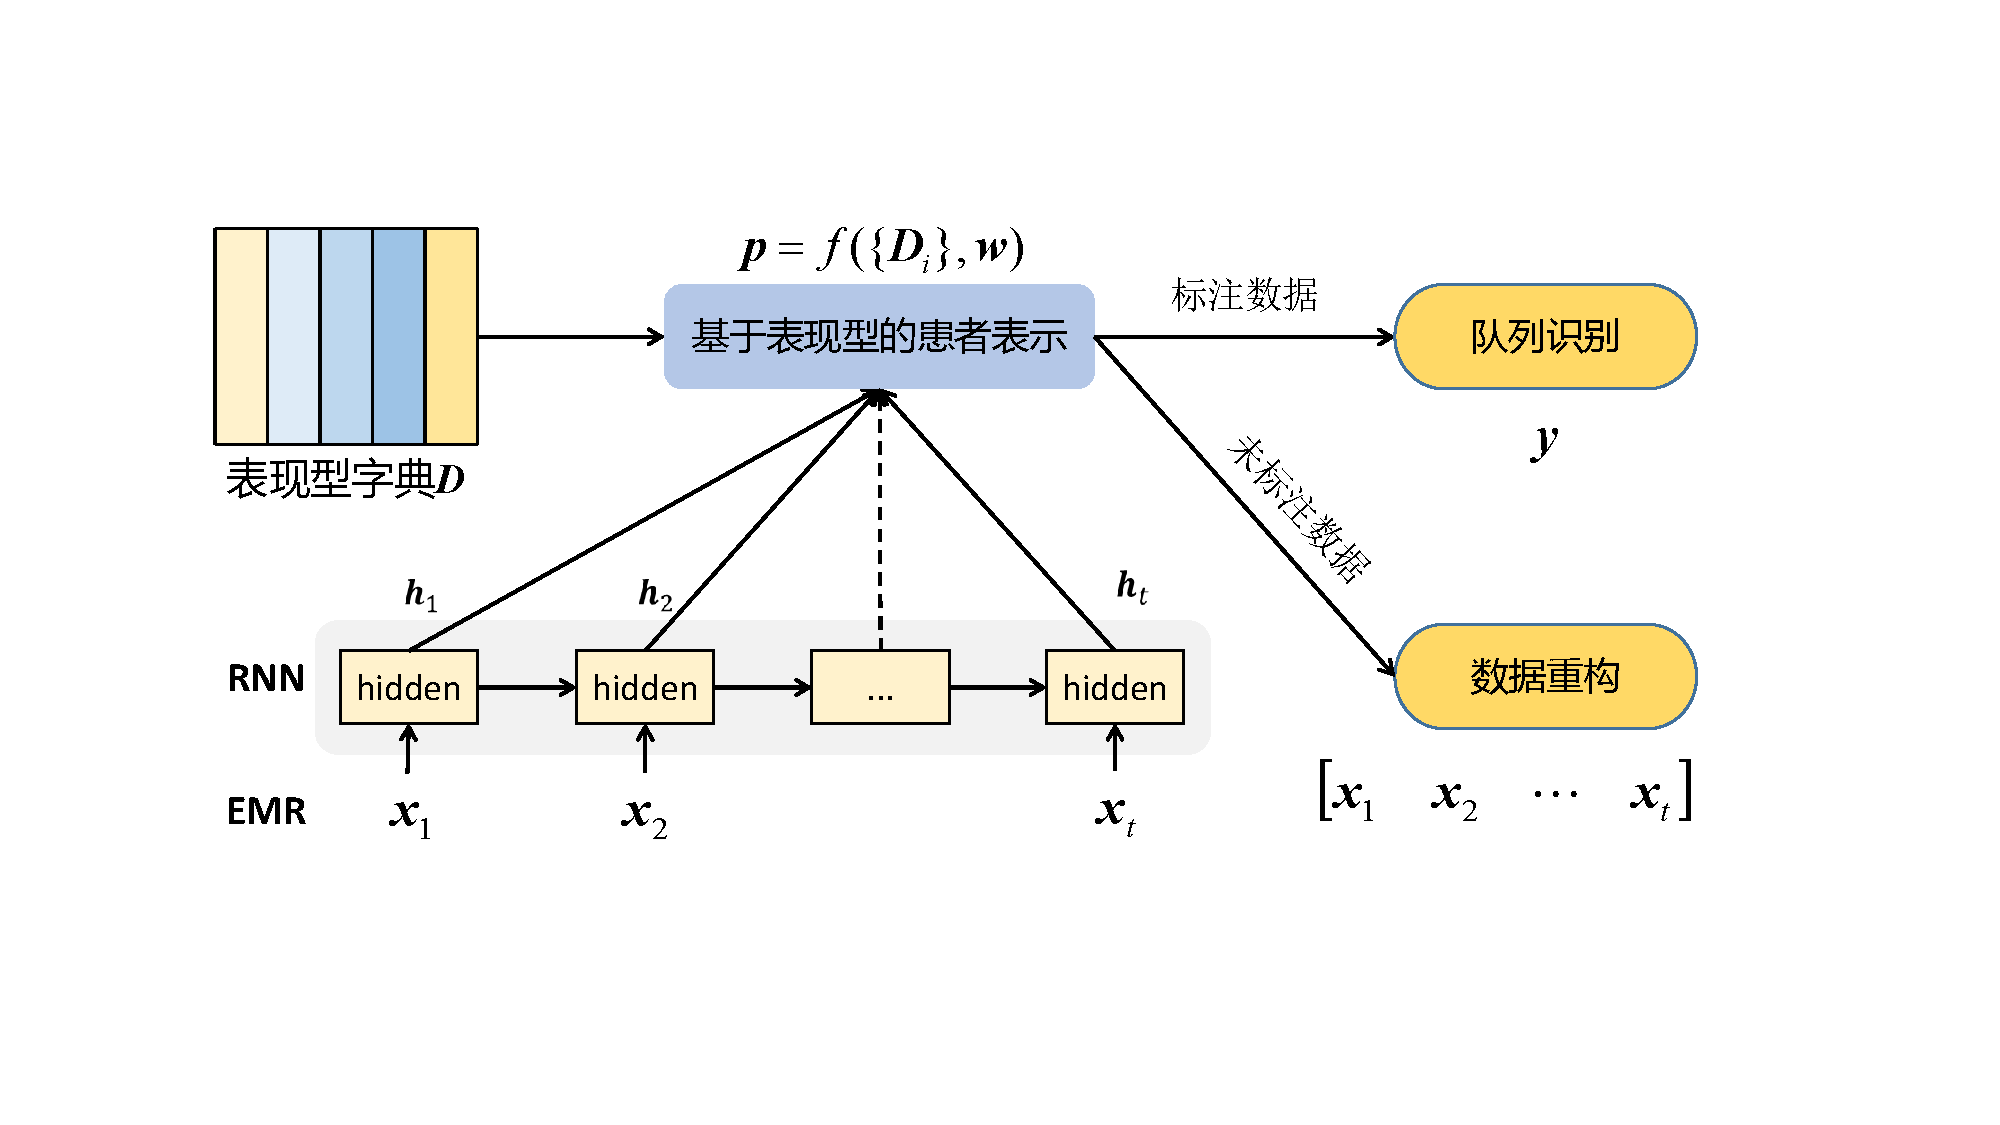
\includegraphics[width=0.8\textwidth]{ch3CI.pdf}
        \end{center}
        \caption{基于表现型的自动队列识别研究方案}
        \label{fig:ch3:ci}
    \end{small}
\end{figure}

现有电子医疗记录表示学习的工作主要学习医疗特征向量和患者某次就医向量,尚没有针对
表现型的向量表示学习。相比于现有工作,本方案可对患者的向量表示进行分解,得到各个
患者共享的表现型字典向量,保留患者语义信息用于重构任务。此外,本项目还将从以下两
方面进一步改进模型:
\begin{itemize}
    \item 利用\textbf{标签嵌入(label embedding)的方法,建立队列识别目标$\bm y$
    和表现型字典的映射关系},提高了队列识别的准确性和模型的可解释性;
    \item \textbf{引入医疗领域与表现型相关的知识库},如
    PheKB~\footnote{https://phekb.org/phenotypes},构建表现型字典和领域知识库的
    映射关系,并利用知识库作为模型训练的约束条件,引导表现型向量训练。
\end{itemize}



\subsubsection{融合医学偏差的EMR自动插补}\label{ch3_2}

\begin{comment}
融合医学偏差的EMR自动插补旨在将在时间维度上不规则的电子医疗记录补全为完整的电子
医疗记录,可降低后续预测模型的复杂度和训练时间。电子医疗记录除了反映患者的身体健
康状态,还包含的患者与医院、医生与电子病历系统的交互过程,通常这些附加因素会引入
医学偏差。研究表明,医学偏差可用于对患者更精细的分类,对于理解电子医疗记录有重要
辅助作用,许多医学偏差都会通过医疗特征被记录的时间推断出来,这为建模引入医学偏差
提供了理论基础。本项目利用医疗特征记录的时间和电子医疗记录中缺失值出现的位置,学
习特征的缺失规律,进而将所学缺失规律融入插补模型中。
\end{comment}

\begin{figure}
    \begin{small}
        \begin{center}
            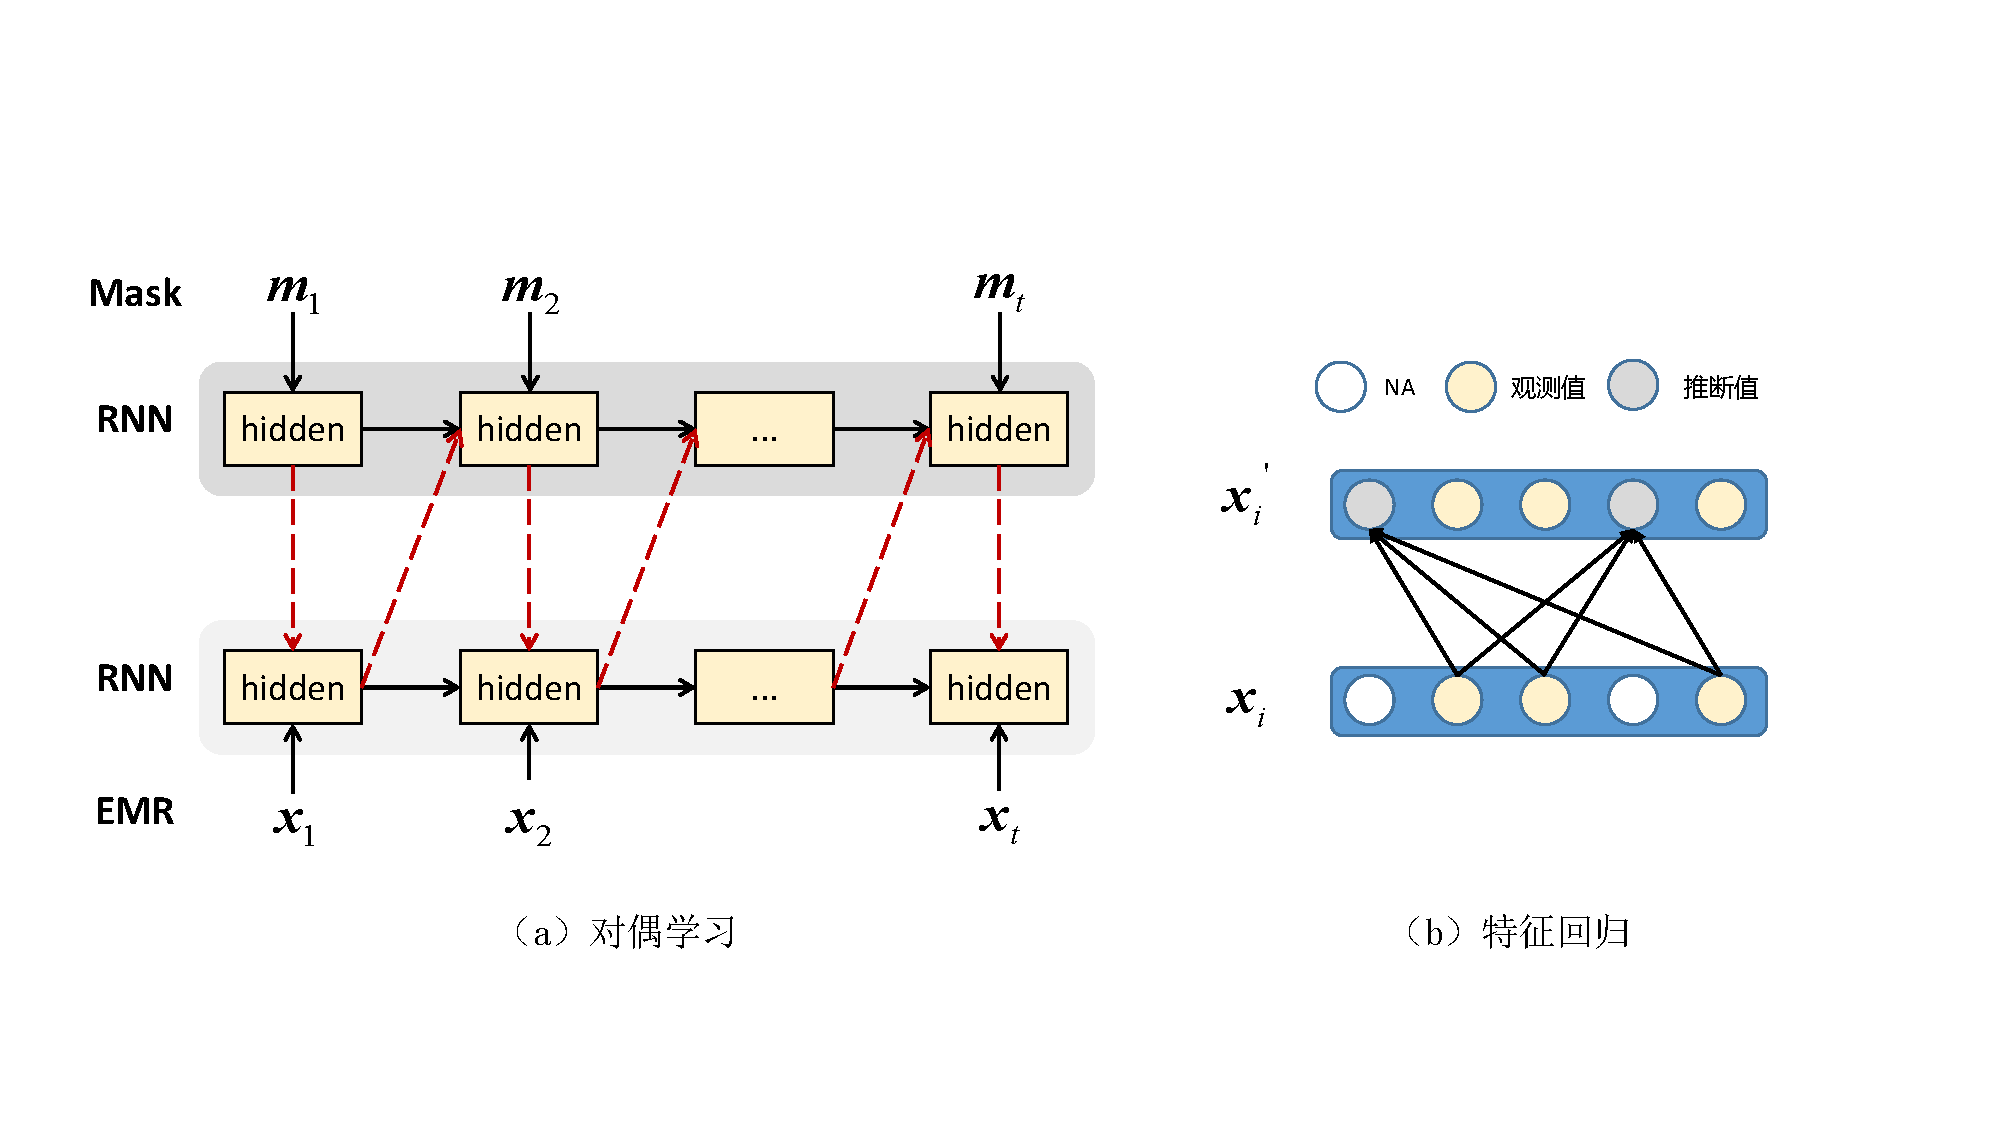
\includegraphics[width=0.95\textwidth]{ch3imputation.pdf}
        \end{center}
        \caption{融合医学偏差的EMR自动插补研究方案}
        \label{fig:ch3:imputation}
    \end{small}
\end{figure}

本项目EMR插补的核心模块如\cref{fig:ch3:imputation}所示。首先,本项目拟针对缺失标
记(即图中的$(\bm m_1, \bm m_2, \dots, \bm m_t)$)建模,如
\cref{fig:ch3:imputation} (a)所示,缺失标记可以反映特征是否被记录,通过对缺失标
记建模,可以得到各个医疗特征在不同时间的缺失规律,即患者医疗特征被记录的规律。同
时,本项目对已经观察到的医疗记录进行建模,这也是缺失值插补最重要的推断基础。我们
发现,在电子医疗记录中,\textbf{缺失矩阵$(\bm m_1, \bm m_2, \dots, \bm m_t)$和观
察到的数据$(\bm x_1, \bm x_2, \dots, \bm x_t)$具有对偶关系},即缺失标记和观测数
据是相互影响的,可作为互相取值推断的参考。以新冠肺炎为例,按照国家卫健委制定的诊
断标准,如果患者2次核酸检测为阴性,则证明其已经康复,所以接下来短时间内患者的核
酸检测结果将会缺失,反之,在医疗条件具备的情况下,如果患者长时间没有被安排核酸检
测,则该患者很可能没有患病,核算检测结果也较大概率为阴性。因此,本项目拟通过对偶
学习方法,融合缺失矩阵和数值矩阵对缺失值进行推测。

其次,电子医疗记录包含多元特征,特征之间一般具有潜在的相互关系,为插补合理的缺失
值,应考虑特征之间的相互关系。如\cref{fig:ch3:imputation} (b)所示,本项目拟在建
模过程中引入\textbf{特征回归}方法,以深度学习模型对特征间关系进行建模,在统一时
间点,若以观察到部分数据,可用它们推断缺失值,这种方法被称为特征回归。
\cref{fig:ch3:imputation} (b)展示的特征回归建模为一个线性层,可以建模为$\bm
x_i^{\prime} = f(\bm W, \bm b; \bm x) = \bm{Wx_i}+\bm b$。

最后,由于不同特征记录时间的差异性,电子医疗记录还具有特征层面的不规则性,即不同
特征的记录时间、记录频率差别很大,所以直接使用原始RNN模型进行EMR插补容易丢失特征
在时间维度方面的信息,因此,本项目拟通过修改GRU(Gated Reccurent Unit)的门机
制,在GRU中引入时间衰减因子,通常而言,特征记录时间离当前时间越远,对患者当前的
状态影响越小,反之,特征记录时间离当前时间越近,则对患者当前的状态影响更大。通过
在GRU中引入时间衰减因子,可以细腻度的控制特征层面的不规则性带来的影响。


\subsubsection{结合特征重要性和时间关联性的可解释预测模型}\label{ch3_3}

电子医疗记录中包含静态特征(如:性别、籍贯等)和动态特征(如:血糖值、慢性肾病分
期等),显然,静态特征随着时间的推移不会发生变化,因此,本项目在构建预测模型时拟
首先针对静态特征和动态特征分别建模,然后将两组特征的向量表示融合起来。

预测模型的可解释性对于临床应用具有重要意义,就电子医疗记录预测性分析而言,模型的
可解释性可以具体化为两方面:1)对于给定研究队列和模型,分析特征的重要性,称为模
型的\textbf{全局可解释性};2)对于某个样本的预测结果,\textbf{提供导致该结果的主
要因素},即一个或者一组具体时间的具体特征值。

由于电子医疗记录中的静态特征远少于动态特征,特征维度较低,本项目拟采取单层全连
接神经网络进行建模,有助于直接计算特征的重要性。对于单个样本预测结果的解释,本项
目拟通过\textbf{深度泰勒分解(Deep Taylor Decomposition)}算法~\citess{montavon2017explaining}分析分析静态特征对预测结果的贡献。对动态特征,本
项目拟采用RNN模型进行建模,虽然RNN能有效捕捉电子医疗记录中的长时间依赖的关系,但
由于其隐含层多次计算,且参数复用,难以通过现有方法得到特征的重要性和具体记录的重
要性。\textbf{本项目拟设计混合注意力机制,解耦时序模型中特征的相互关系和时间的依
赖性}。

\cref{fig:ch3:interpretability}是本项目针对动态特征的可解释性研究方案的示意图,
以图中描述的2个特征为例,首先,为了解耦隐含层是由多个特征计算得到的,我们对输入
$\bm x_i$的每个特征分别计算其隐层表示,然后以拼接的形式组成$\bm x_i$的隐含表示
$\bm h_i = [\bm h_{i1}, \bm h_{i2}]$,这样分开训练虽然避免了特征组合对可解释性的
影响,但这样做会降低模型预测的准确率,本方案利用混合注意力机制实现特征自动组合和
转换,在提高模型可解释性时,也不影响预测性能。

\begin{figure}
    \begin{small}
        \begin{center}
            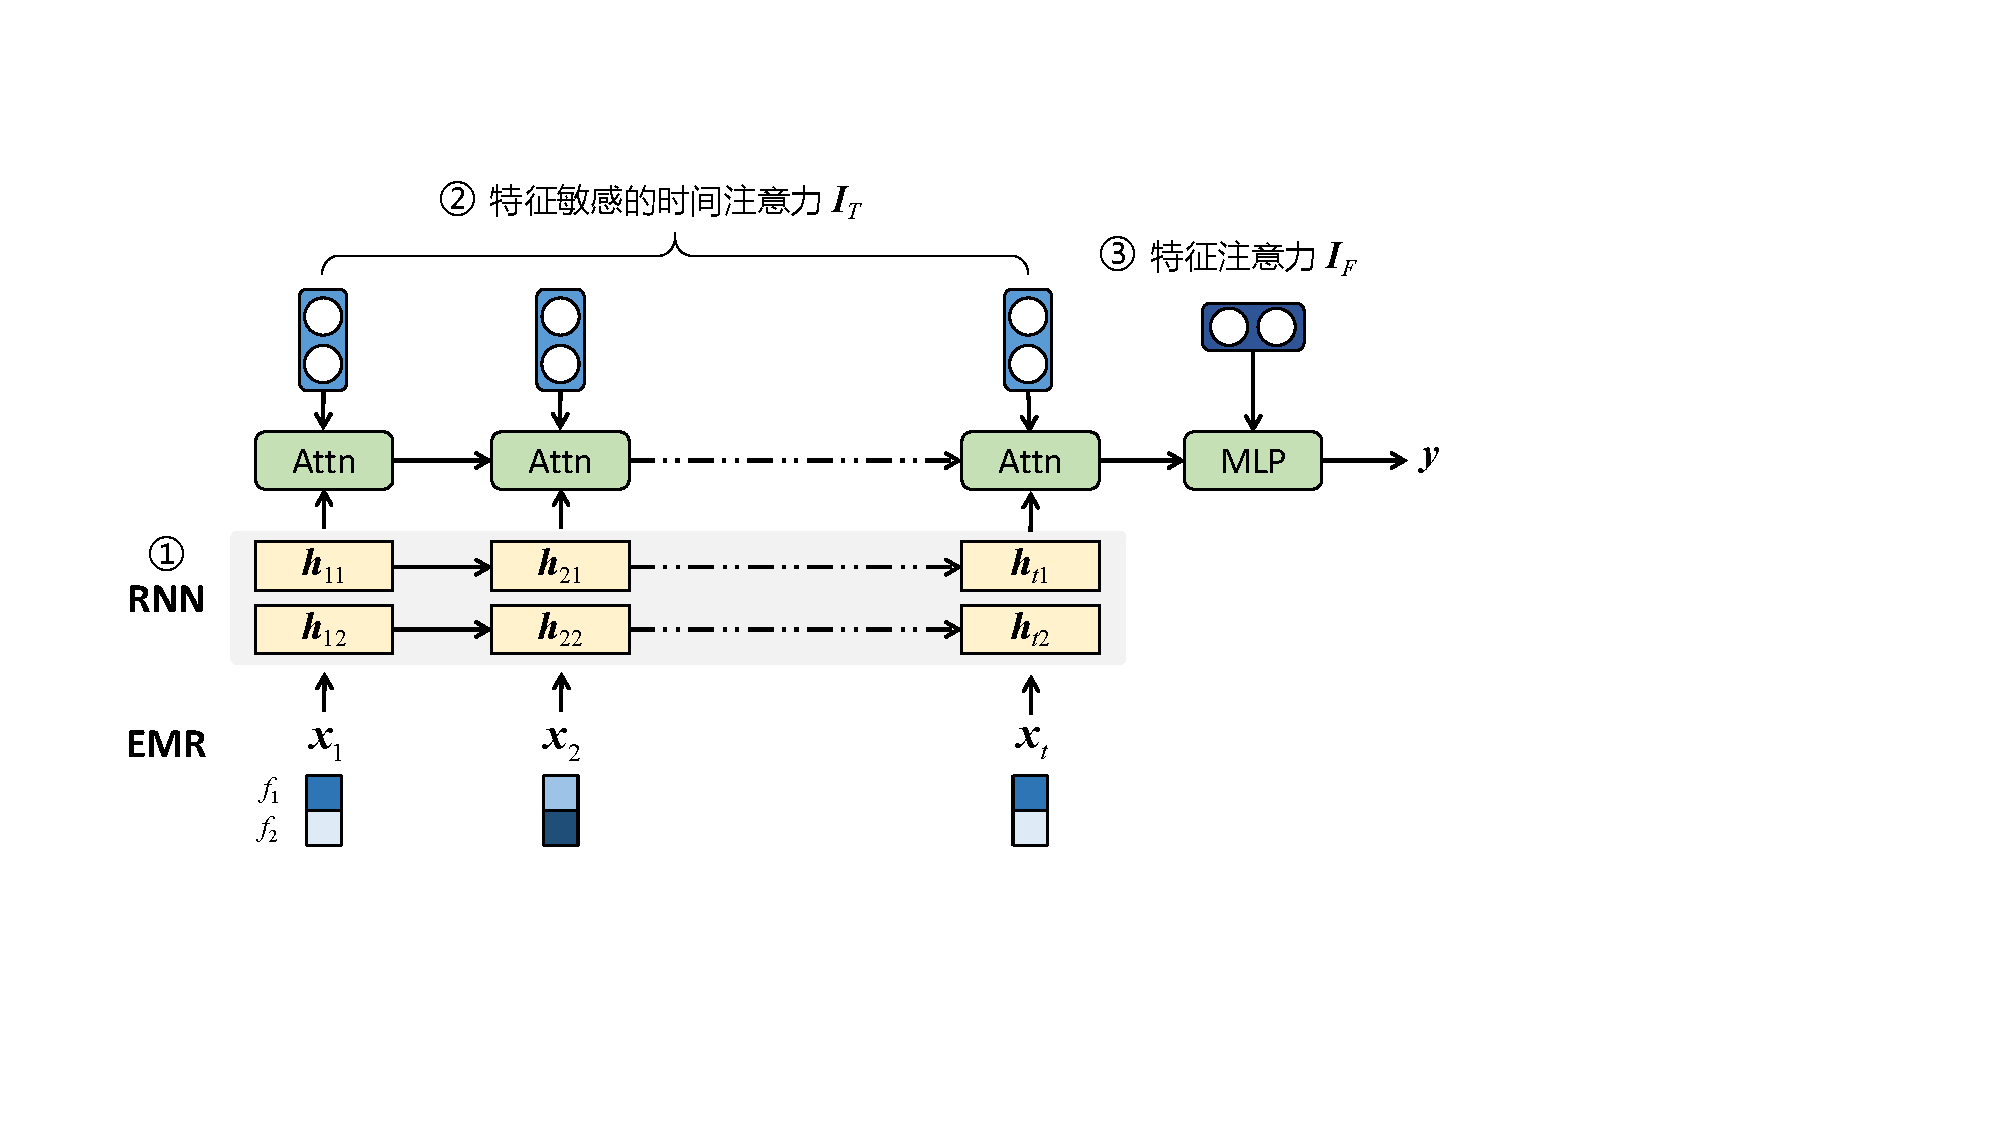
\includegraphics[width=0.85\textwidth]{ch3interpretability.pdf}
        \end{center}
        \caption{可解释预测模型(动态特征)研究方案}
        \label{fig:ch3:interpretability}
    \end{small}
\end{figure}

\textbf{本方案的混合注意力机制包括特征敏感的时间注意力和特征注意力两部分,特征敏
感的时间注意力参数为$\bm I_T \in \mathbb R^{v \times t}$,其中$v$表示特征的个
数,$t$代表时间点的个数}。输入$\bm x_i$的隐含层表示$\bm h_i$通过图中所示的时间注
意力模块(Attn)进行特征融合,具体而言,时间注意的模块的输出为$\bm I_{T_i} \odot
\bm h_i$,其中$\odot$表示沿着时间维度利用特征隐向量乘以注意力权重,即$\bm
I_{T_i} \odot \bm h_i= \sum_{j=1}^v I_{T_{ij}} \bm h_{ij}$。通过引入特征敏感的时
间注意力权重,可学习每个特征在不同时间点(即每条记录)的重要性,而特征注意力参数
$\bm I_F \in \mathbb R^{v}$则用于学习特征的对于模型和预测结果整体重要性,在最后
的全连接层之前与静态特征表示融合并引入模型,以便实现静态特征和动态特征的统一比
较。在此框架下,动态特征的可解释性可建模为以下形式:

\begin{equation}
    \begin{aligned}
        p(\bm y | \bm X) =& \sum_{i=1}^v p(y|z=i, \bm X) P(z=i | \bm X) \\
            =& \sum_{i=1}^v p(y|z=i, I_{T_{1i}} \cdot \bm h_{1i}, I_{T_{2i}} \cdot \bm h_{2i}, \dots, I_{T_{ti}} \cdot \bm h_{ti}) \\
            & \cdot P(z=i|I_{F_1} \cdot \bm h_{t1}, I_{F_2} \cdot \bm h_{t2} \dots, I_{F_v} \cdot \bm h_{tv})
    \end{aligned}
\end{equation}
其中$\bm X= (\bm x_1, \bm x_2, \dots, \bm x_t)$为模型输入,$z$是隐变量,表示数据
特征的编号,$z \in {1,2,\dots, v}$,用于解释不同特征的重要性和时间关联性。
$I_{T_{1i}} \cdot \bm h_{1i}, I_{T_{2i}} \cdot \bm h_{2i}, \dots, I_{T_{ti}}
\cdot \bm h_{ti}$即为特征$i$时间维度的注意力,而$P(z=i|I_{F_1} \cdot \bm h_{t1},
I_{F_2} \cdot \bm h_{t2}, \dots, I_{F_v} \cdot \bm h_{tv})$则为特征$i$的全局重要
性。

\subsubsection{临床预测性任务}

从DKD慢性肾病和急诊科感染性休克的临床需求出发,利用本项目的研究成果,研发预测分
析系统:

首先,熟悉DKD慢性肾病和急诊科感染性休克的医学背景,与医生合作,标注少量符合表现
型的队列数据,利用第(1)节研发的模型从大规模电子医疗记录中筛选出研究队列;其次,
对获得的研究队列进行预处理,分析记录时间分布的特点,利用第(2)节的研究成果对研究
队列进行缺失值补充,并评估数据插补的效果;以第(3)节的核心方法构建可解释预测模
型,评估其预测准确率,并研发特征重要性和时间关联性的可视化系统,展示模型和预测结
果的可解释性分析效果。研究过程中,医生的反馈可作为本项目队列识别、数据插补和可解释模型研究的重要指导,确保本项目研究成果具有实际应用价值。

\subsection{可行性分析}

\subsubsection{理论可行性}

本项目研究目标明确,研究内容清晰,研究方案和技术路线中所应用的方法和技术手段在业
界都有着成熟清晰的理论基础。申请人和项目组对这些关键技术和理论有着深入的了解和掌
握,近年来在人工智能、医疗数据分析等领域的高水平会议上发表了多篇论文。项目组前期
已经对本项目中提到的研究内容分别进行了详细的调研和分析,并在医疗特征表示学习、时
间序列插补等领域取得了初步成果。因此,从理论上说,本项目是可行的。

\subsubsection{技术可行性}

申请人前期调研了大量基于深度学习的电子医疗记录分析的研究工作(如
\ref{relatedwork}节所述),深度学习模型不仅能挖掘高维特征之间复杂的关系,同时能
有效处理数据中长时间依赖关系,非常适合电子医疗记录分析。利用深度学习技术解决电子
医疗记录预测性分析需要解决三个核心问题,即队列识别、EMR不规则性处理和模型的可解
释性,申请人之前的研究工作一直聚焦于电子医疗记录的分析,在医疗特征表示学习、多元
时序数据插补等方面已取得一定的研究成果,并在攻读博士期间与医生合作,参与过医疗分
析系统的开发,相关研发经验可作为本项目的研究基础。申请人所在项目组多年来一直活跃
在在大数据处理和分析、机器学习等领域,在相关领域有着丰富的研究经验和技术积累。同
时,在研究过程中,申请人与医疗机构建立了合作关系,积累了大量可用于实验的真实数据
集。因此,从技术上说,本项目是可行的。

\subsubsection{团队合理性}

项目组在大数据分析和人工智能领域具有一定的基础,积累了丰富的研究经验,在重要国际
会议上发表了多篇高水平论文,项目在信息系统和数据分析系统开发方面也有丰富的积累,
可为本项目可视化分析系统研发提供保障。项目组梯队完善,队伍具有凝聚力和创造力,项
目组成员每周定期讨论,有着良好的科研氛围,同时对本项目的研究内容具有浓厚的研究兴
趣。申请人与联合培养时的导师新加坡国立大学教授Beng Chin Ooi(黄铭钧)一直保持密
切联系,Ooi教授长期研究大数据管理与分析,是数据库和数据挖掘方面非常活跃的科学
家,可为本项目提供技术指导。

申请人与医疗机构和专家一直保持良好的合作关系,与北京大学医疗健康大数据国家研究院
张路霞教授合作研究慢性肾病患者病情进展,和天津市肿瘤医院合作研究肺癌患者治疗效果
评估,同时,申请人参与建设“南开大学-基准联合医学研究中心”,和广州基准医疗有限公
司合作研究基于多模态医疗数据的癌症早诊技术。这些合作单位和专家可为本项目提供专业
意见的反馈,保证研究内容符合医学常识和临床需求。综上所述,项目团队组成合理,能保
障本项目的顺利完成。